As mentioned above, the triangulation step of the time-frequency method fails for source azimuths of $|\varphi_0| = 90^\circ$.
Consequently, for this method only, we have varied the source azimuth only from $\varphi_0 = 0^\circ$ to $85^\circ$ in increments of $5^\circ$ and averaged over these azimuths.

% Level

In \figref{fig:09_Thiergart_Comparison:Level_Errors:Thiergart}, we plot the level errors (as defined in \secref{sec:04_Auditory_Models:Audible_Energy}) incurred by the time-frequency method as a function of array spacing $\Delta$ and normalized source distance $\gamma$.
For ease of comparison with the proposed navigational method, in this section we have reproduced the corresponding contour plots (e.g., \figref{fig:09_Thiergart_Comparison:Level_Errors:Hybrid}) from \secref{sec:08_Proposed_Method:Results}.
From \figref{fig:09_Thiergart_Comparison:Level_Errors:Thiergart}, we see that the time-frequency method is able to achieve approximately zero error almost everywhere, with the exception of far interior sources ($\gamma < 1$).
This yields an improvement over the proposed method, which is only able to accurately reconstruct the sound level for exterior sources ($\gamma > 1$) and is otherwise several dB too quiet for interior sources.

\begin{figure*}[t]
	\centering
	\begin{subfigure}[b]{0.49\textwidth}
		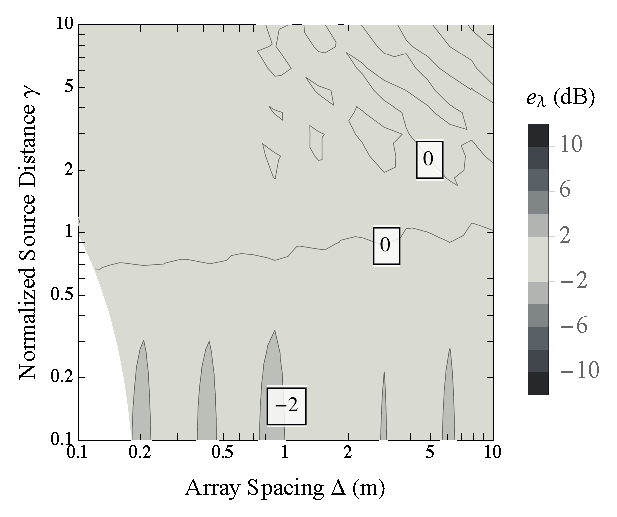
\includegraphics[width=\textwidth]{09_thiergart_comparison/figures/audibleEnergy_contour_thiergart.eps}
		\caption{\citet{Thiergart2013} method}
		\label{fig:09_Thiergart_Comparison:Level_Errors:Thiergart}
	\end{subfigure}
	\hfill
	\begin{subfigure}[b]{0.49\textwidth}
		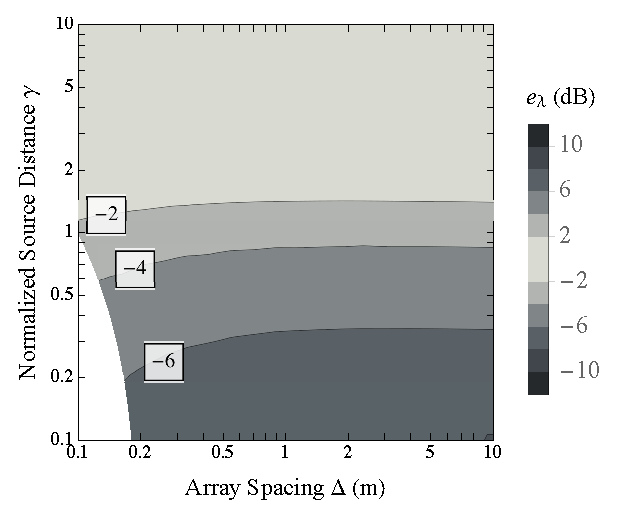
\includegraphics[width=\textwidth]{08_proposed_method/figures/audibleEnergy_contour_validhybrid.eps}
		\caption{Proposed method}
		\label{fig:09_Thiergart_Comparison:Level_Errors:Hybrid}
	\end{subfigure}
	
	\caption[Contour plots of level errors for each interpolation method.]{
	Level errors $e_\lambda$ for microphone spacing $\Delta$ and normalized source distance $\gamma$.
  Contour lines are drawn every $2$~dB.
  \Figref{fig:09_Thiergart_Comparison:Level_Errors:Hybrid} has been reproduced from \figref{fig:08_Proposed_Method:Level_Errors:Hybrid}.}
	\label{fig:09_Thiergart_Comparison:Level_Errors}
\end{figure*}

% Coloration

For spectral coloration, however, we see in \figref{fig:09_Thiergart_Comparison:Spectral_Errors:Thiergart} that the time-frequency method yields larger spectral errors (as defined in \secref{sec:04_Auditory_Models:Coloration_Metrics:ABSE}) than the proposed method for all microphone spacings larger than approximately $0.5$~m.
In particular, the proposed method yields significantly smaller errors for interior sources with large microphone spacings ($\gamma < 1$ and $\Delta > 0.5$~m).
Only for exterior sources with microphone spacings smaller than approximately $0.25$~m does the time-frequency method achieve smaller spectral errors than the proposed method.
As the precise origin of the spectral coloration induced by translation via the time-frequency method remains unclear, future investigations should attempt to determine the source of, and ideally correct for, such colorations.

\begin{figure*}[t]
	\centering
	\begin{subfigure}[b]{0.49\textwidth}
		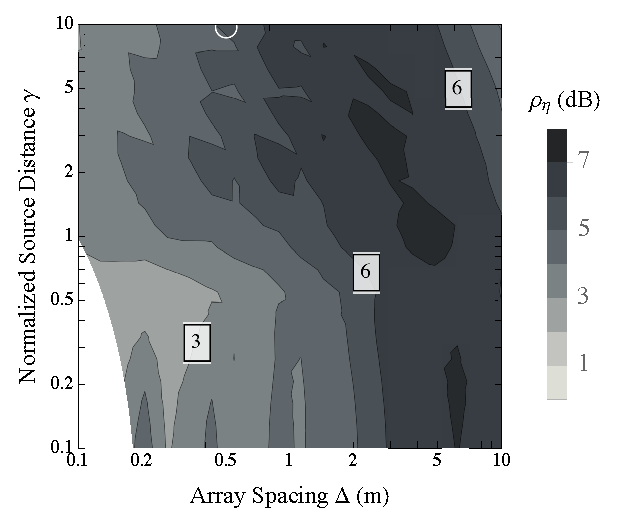
\includegraphics[width=\textwidth]{09_thiergart_comparison/figures/scharer2009_contour_thiergart_marked.eps}
		\caption{\citet{Thiergart2013} method}
		\label{fig:09_Thiergart_Comparison:Spectral_Errors:Thiergart}
	\end{subfigure}
	\hfill
	\begin{subfigure}[b]{0.49\textwidth}
		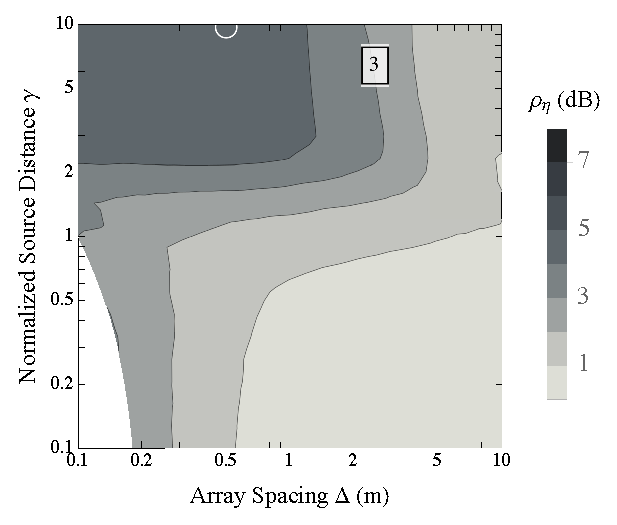
\includegraphics[width=\textwidth]{09_thiergart_comparison/figures/scharer2009_contour_validhybrid_marked.eps}
		\caption{Proposed method}
		\label{fig:09_Thiergart_Comparison:Spectral_Errors:Hybrid}
	\end{subfigure}
	
	\caption[Contour plots of spectral errors for each interpolation method.]{
	Spectral errors $\rho_\eta$ for microphone spacing $\Delta$ and normalized source distance $\gamma$.
  Contour lines are drawn every $1$~dB.
  The white semicircles indicate the conditions shown in \figref{fig:09_Thiergart_Comparison:Azimuth_Dependence}, where $\Delta = 0.5$~m and $\gamma = 10$.
  \Figref{fig:09_Thiergart_Comparison:Spectral_Errors:Hybrid} has been reproduced from \figref{fig:08_Proposed_Method:Spectral_Errors:Hybrid}.}
	\label{fig:09_Thiergart_Comparison:Spectral_Errors}
\end{figure*}

Recalling the discussion in \secref{sec:09_Thiergart_Comparison:Azimuth_Dependence}, we now see that the spectral errors corresponding to the conditions shown in \figref{fig:09_Thiergart_Comparison:Azimuth_Dependence} (with $\Delta = 0.5$~m and $\gamma = 10$) are indeed comparable:
at that point in \figreftwo{fig:09_Thiergart_Comparison:Spectral_Errors:Thiergart}{fig:09_Thiergart_Comparison:Spectral_Errors:Hybrid}, the time-frequency method yields a spectral error of approximately 5~dB and the proposed method yields a spectral error between 4 and 5~dB.
To understand this apparent discrepancy between \figreftwo{fig:09_Thiergart_Comparison:Azimuth_Dependence}{fig:09_Thiergart_Comparison:Spectral_Errors}, it should be recalled that the spectral error calculation effectively ``smooths'' the frequency responses via averaging over a bank of gammatone filters (see \eqnref{eq:ABSE}).
It should also be emphasized that the frequency response plots shown in \figref{fig:09_Thiergart_Comparison:Azimuth_Dependence} only illustrate a single condition ($\Delta = 0.5$~m, $\gamma = 10$, and $\vec{r}_0 = (0,0,0)$), whereas the data shown in \figref{fig:09_Thiergart_Comparison:Spectral_Errors} have been averaged over the entire navigable region and all source azimuths.

% Localization

Localization errors (as computed with \eqnref{eq:04_Auditory_Models:Localization_Error} for the localization model described in \secref{sec:05_Proposed_Models:Localization_Model}) for the time-frequency method are shown in \figref{fig:09_Thiergart_Comparison:Localization_Errors:Thiergart}.
Contrary to that method's coloration performance (see \figref{fig:09_Thiergart_Comparison:Spectral_Errors:Thiergart}), which is most accurate at small microphone spacings (e.g., $\Delta < 0.5$~m), the localization errors incurred by this method are largest at those small microphone spacings.
In particular, for exterior sources with microphone spacings smaller than approximately $0.3$~m, the proposed method yields a significant improvement ($\sim15^\circ$) over the time-frequency method.
Additionally, for far exterior sources ($\gamma > 3$) and at all microphone spacings, the proposed method yields a reasonably large improvement ($\sim5^\circ$) over the time-frequency method.
For microphone spacings larger than approximately $0.5$~m, the errors incurred by the proposed method are relatively constant with spacing, whereas those incurred by the time-frequency method improve with increasing spacing and even become very small ($\epsilon_\nu < 5^\circ$) at large $\Delta$ and $\gamma < 1$.
Accordingly, the time-frequency method yields a significant improvement over the proposed method for interior sources with microphone spacings larger than approximately $1$~m.

\begin{figure*}[t]
	\centering
	\begin{subfigure}[b]{0.49\textwidth}
		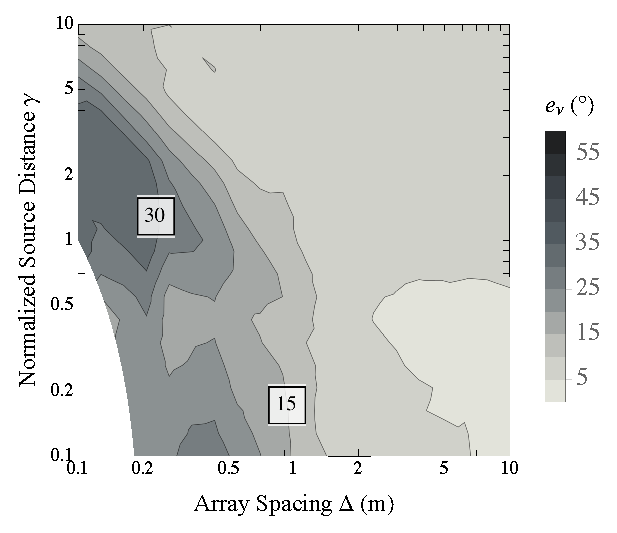
\includegraphics[width=\textwidth]{09_thiergart_comparison/figures/tylka2017_contour_thiergart.eps}
		\caption{\citet{Thiergart2013} method}
		\label{fig:09_Thiergart_Comparison:Localization_Errors:Thiergart}
	\end{subfigure}
	\hfill
	\begin{subfigure}[b]{0.49\textwidth}
		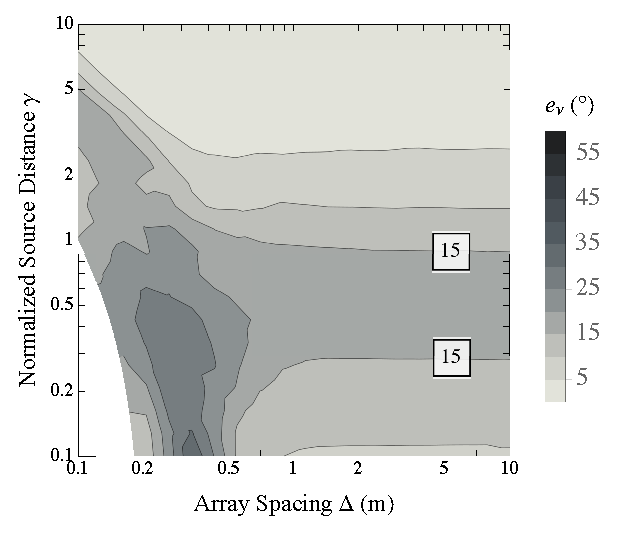
\includegraphics[width=\textwidth]{08_proposed_method/figures/tylka2017_contour_validhybrid.eps}
		\caption{Proposed method}
		\label{fig:09_Thiergart_Comparison:Localization_Errors:Hybrid}
	\end{subfigure}
	
	\caption[Contour plots of localization errors for each interpolation method.]{
	Predicted localization errors $e_\nu$ for microphone spacing $\Delta$ and normalized source distance $\gamma$.
	Contour lines are drawn every $5^\circ$.
	\Figref{fig:09_Thiergart_Comparison:Localization_Errors:Hybrid} has been reproduced from \figref{fig:08_Proposed_Method:Localization_Errors:Hybrid}.}
	\label{fig:09_Thiergart_Comparison:Localization_Errors}
\end{figure*}

% Diffuseness

From the plots of diffuseness errors (see \secref{sec:04_Auditory_Models:Diffuseness_Parameter}) shown in \figreftwo{fig:09_Thiergart_Comparison:Diffuseness_Errors:Thiergart}{fig:09_Thiergart_Comparison:Diffuseness_Errors:Hybrid}, we immediately see that the proposed method achieves more accurate performance than the time-frequency method over all conditions.
The time-frequency method consistently yields a diffuseness parameter which is too small, whereas the proposed method achieves nearly exact diffuseness (except at very small $\gamma$ and $\Delta$).

\begin{figure*}[t]
	\centering
	\begin{subfigure}[b]{0.49\textwidth}
		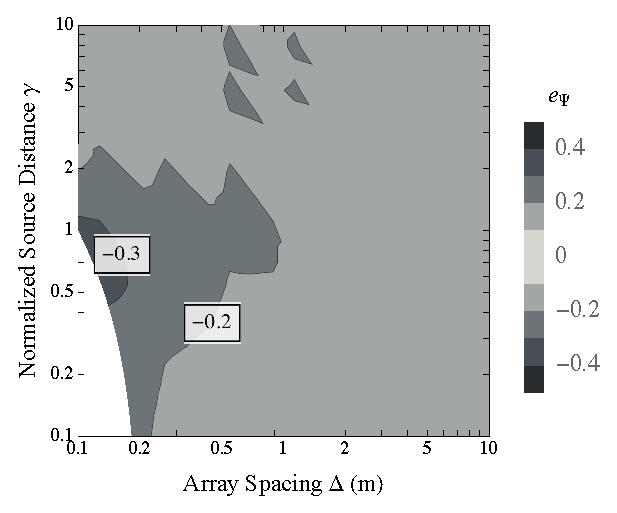
\includegraphics[width=\textwidth]{09_thiergart_comparison/figures/merimaa2005_d_contour_thiergart.eps}
		\caption{\citet{Thiergart2013} method}
		\label{fig:09_Thiergart_Comparison:Diffuseness_Errors:Thiergart}
	\end{subfigure}
	\hfill
	\begin{subfigure}[b]{0.49\textwidth}
		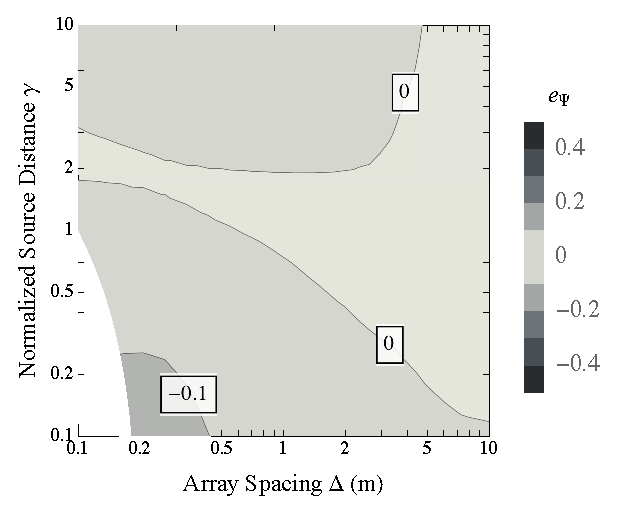
\includegraphics[width=\textwidth]{08_proposed_method/figures/merimaa2005_d_contour_validhybrid.eps}
		\caption{Proposed method}
		\label{fig:09_Thiergart_Comparison:Diffuseness_Errors:Hybrid}
	\end{subfigure}
	
	\caption[Contour plots of diffuseness errors for each interpolation method.]{
	Diffuseness errors $e_\Psi$ for microphone spacing $\Delta$ and normalized source distance $\gamma$.
  Contour lines are drawn in increments of $0.1$.
  \Figref{fig:09_Thiergart_Comparison:Diffuseness_Errors:Hybrid} has been reproduced from \figref{fig:08_Proposed_Method:Diffuseness_Errors:Hybrid}.}
	\label{fig:09_Thiergart_Comparison:Diffuseness_Errors}
\end{figure*}

This apparent deficiency in diffuseness of the time-frequency method suggests that the diffuse sound term in the sound field re-synthesis equation, \eqnref{eq:03_Navigation_Techniques:Thiergart_Synthesis}, is underestimated by the method.
Consequently, it may be relatively straightforward to modify the time-frequency method to correct for this behavior.
This is a topic for further development.